\documentclass[draft]{article}
\usepackage{fixme}
\usepackage{graphicx}
\usepackage[utf8x]{inputenc}
\usepackage{url}
\usepackage{acronym}
\usepackage{tikz}
\usepackage{bm}
\usepackage{subcaption}
\usepackage{listings}
\usepackage[section]{placeins}
\usepackage{etoolbox}
\preto\section\acresetall
\usetikzlibrary{calc,positioning,shapes,decorations.pathreplacing}

\tikzset{
short/.style={draw,rectangle,text height=3pt,text depth=13pt,
  text width=7pt,align=center,fill=gray!30},
long/.style={short,text width=1cm},
double/.style={short,text width=2cm}
}



\begin{document}
% the long nodes \lnode{<label>}{<right of>}
\def\snode#1#2#3{%
  \node[long,right=of #1, label=center:#3] (#2) {}}

\def\dnode#1#2#3{%
  \node[double,right=of #1, label=center:#3] (#2) {}}


\begin{titlepage}
	\begin{center}
   	{\scshape\LARGE
    	Department of Information Engineering and Computer Science\\
      	(DISI)\\
      	University of Trento, Italy\\\par}
      	\vspace{1cm}
      	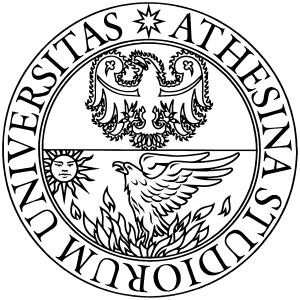
\includegraphics[scale=0.35]{logo}\\
	\vspace{1cm}
	{\scshape\Large Network Security - AY 2017/2018 \par}
	\vspace{1cm}
	{\huge\bfseries Lab Activity Report\\\par}
	\noindent\makebox[\linewidth]{\rule{\linewidth}{0.4pt}}
	{\Large\bfseries Man in the Middle attacks\par}
      	\noindent\makebox[\linewidth]{\rule{\linewidth}{0.4pt}}

        \vspace{.5cm}
        Author: \\
       	Gabriele Gemmi [198042] \\
				Lorenzo Brugnera [197054]
      	\vfill
      	\vfill
	\end{center}
\end{titlepage}

\section{Introduction}
\acrodef{MitM}{Man in the Middle}
\paragraph{What are \ac{MitM} attacks}
A man in the Middle attack is an attack where the attacker secretly relays
and possibly alters the communication between two parties who believe they
are directly communicating with each other. The aim of the attacker is to
take the control of the communication and to intercept all relevant messages
passing between the two victims. \\
Once the attacker puts himself ``\textit{in the middle}'', he can do eavesdropping,
which means secretely listening to a private conversation of other parties without their consent.
This type of attack is very effective when the connection between the two
victims is not secure (HTTP).
In this way, all the traffic is exchanged in clear and the attacker can
easily manage to intercept sensitive data, like usernames, passwords, cookies and so on. \\
A \ac{MitM} attack can be performed on secure connections as well,
with the only difference that the attacker has to establish
two independent SSL sessions, one for each TCP connection.
Generally, browsers handle this kind of things,
notifying the user that the certificate is not valid. \\
A \ac{MitM} is well represented by the following image:

\begin{figure}[h]
\center
\includegraphics[width=.8\textwidth]{../figures/mitm_diagram}
\caption{Diagram of a \ac{MitM} attack}
\end{figure}

\noindent There are several ways to mount a \ac{MitM},
but one important requisite is that the attacker must be ``close''
to the victims, more precisely in the same local network.

\subsection{Network attacks}

\begin{itemize}
  \item ARP poisoning
  \item DHCP (DHCPv6) poisoning
  \item Evil Twin
\end{itemize}

\subsection{Service attacks}
\subsubsection{ARP Poisoning}
\fxnote{Too many repetition of ARP}
\acrodef{ARP}{Address Resolution Protocol}
The \ac{ARP} is a communication protocol used to discover link layer addresses,
such as a MAC addresses, associated with a given network layer address, which is typically IPv4.
This mapping between MAC and IP addresses is a critical function in the Internet protocol suite. \\
\ac{ARP} poisoning is a technique by which an attacker sends spoofed \ac{ARP} messages
onto a local area network with the purpose to alter the mapping between IP and MAC addresses.
\ac{ARP} spoofing may allow an attacker to intercept data frames on a network, modify the traffic,
or stop all traffic.Often the attack is used as an opening for other attacks,
such as denial of service, man in the middle, or session hijacking attacks.
The basic principle behind \ac{ARP} poisoning is the exploitation of the the
\ac{ARP} protocol by sending spoofed messages onto the LAN.
\ac{ARP} poisoning attacks can be run from a compromised host on the LAN,
or from an attacker's machine that is connected directly to the target LAN.\\
Generally, the goal of the attack is to associate the attacker's host MAC address
with the IP address of a target host, so that any traffic meant for the target host
will be sent to the attacker's one. The attacker may choose to manipulate the data before
forwarding them or simply  forwarding the packets to the destination in order to sniff private informations.
The following diagram shows the behaviour of the attack:
\begin{figure}[h]
  \center
  \includegraphics[width=.79\textwidth]{../figures/arp_spoofing}
  \caption{ARP Spoofing attack diagram}
\end{figure}
\paragraph{Countermeasures}
Several countermeasures can be adopted to prevent an \ac{ARP} poisoning attack:
\fxnote{We should either do a list of "things" without providing further information or organize it and provide these information for all of them}
\begin{itemize}
  \item \ac{ARP} poisoning proof switches
  \item Port-Based Network Access Control (802.1x), based on the control of the access ports to the LAN. The protocol provides a mechanism to authenticate devices which want to establish a connection to LAN or WLAN network through a switch or a Wi-Fi access point
  \item VPN, based on encryption. A VPN uses not only an encrypted tunnel, but data are encrypted as well
\end{itemize}

\subsubsection{DHCP Poisoning}
\fxnote{Should we write a brief introduction on what is each of these things? ARP, DHCP, SSL, HSTS?}
\acrodef{DHCP}{Dynamic Host Configuration Protocol}
\ac{DHCP} poisoning is a technique which consists in setting up a rogue \ac{DHCP}  server controlled by the attacker.
Each time a client sends a requests to the legit server, the rogue's response is supposed to arrive earlier than the legit one.
When the legit response arrives, it is simply discarded.
The rogue server can spoof the gateway and all the traffic going away from the local subnet will start to flow into the attacker machine.
Then, the attacker forwards the received traffic accordingly, so the host will not notice any disruption in connectivity.
The following diagram explains how the attack works:
\begin{figure}[h]
\center
\includegraphics[width=.8\textwidth]{../figures/dhcp_poisong}
\caption{DHCP poisoning attack diagram}
\end{figure}
\paragraph{Countermeasures}
\fxnote{We should use the same format as before}
Smart switches are one of the best solutions to avoid this kind of attack. They are based on a mechanism which sets a port as trusted or untrusted. As you can see by the following diagram, the router expects to receive DHCP responses only from the real DHCP server, so all the responses which does not come from the legit server are discarded. The following diagram better clarifies the explained behaviour:

\begin{figure}[h]
\center
\includegraphics[width=.8\textwidth]{../figures/dhcp_snooping}
\caption{DHCP snooping diagram}
\end{figure}

\subsubsection{Evil Twin}
An evil twin is a fraudulent Wi-Fi access point (AP) that appears to be legitimate, set up to eavesdrop on wireless communications.
\acrodef{SSID}{Service Set IDentifier}
The rogue access point must have the same \ac{SSID} of the real one and the victim must receive the rogue AP with a stronger signal than the legitimate one.
\fxnote{Explain why two AP could share the same SSID, concept of ESS}

\begin{figure}[h]
  \center
  \includegraphics[width=.8\textwidth]{../figures/evil-twin}
  \caption{Evil Twin attack diagram}
\end{figure}
\paragraph{Countermeasures}\fxnote{same as before}
Usually, a simple authentication (WPA) does not ensure the client that the access point is legitimate, because the attacker just need to discover the key.
The client must authenticate the AP using 802.1x and verify its legitimacy.

\section{Laboratory activity overview}
The following diagram shows up the network topology we set up in order to mount all the attacks we wanted to explain. It is quite simple and composed by:
\begin{itemize}
  \item Victim (Client)
  \item Server
  \item Attacker
  \item Router
\end{itemize}

\fxnote{PARLARE DELLA CONFIGURAZIONE DI OPENWRT, DIRE ANCHE CHE TIPO DI MACCHINE VIRTUALI CI SONO INSTALLATE}

\begin{figure}[h]
  \center
  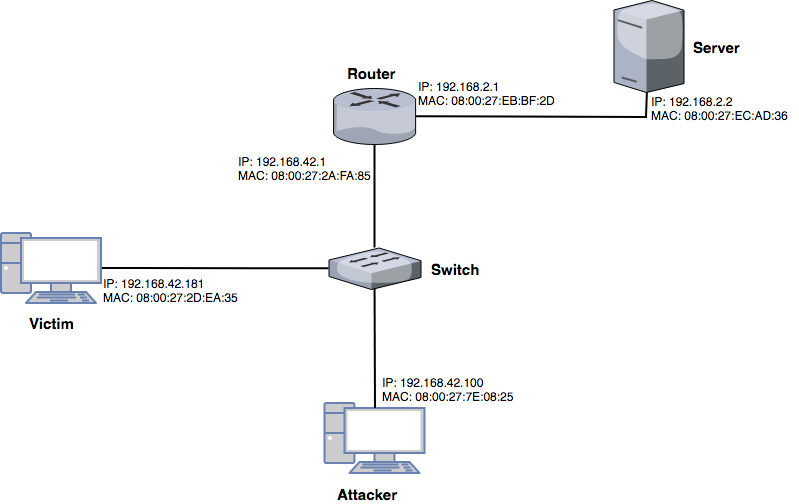
\includegraphics[width=.8\textwidth]{../figures/net_topo}
  \caption{Topology of the VMs network}
\end{figure}
\section{Exercises}

\subsection{Exercise 1 - HTTP Interception}
This first exercise is a very simple one, just to take confidence with the machines.
Basically, in this part you have to capture all the traffic that flows between the victim and the router.
If the traffic is not encrypted, sensitive information can be sniffed by the attacker,
due to the fact that they are exchanged in clear. \\
So, first of all you have to mount a \ac{MitM} network attack:
you can use either any of the attacks we have just illustrated to you or the ettercap\footnote{\url{http://www.ettercap-project.org/ettercap/}} tool.
Because this is a laboratory focusing on \ac{MitM} attacks, for simplicity we will use this simple command line tool available in the dsniff package\footnote{\url{https://www.monkey.org/~dugsong/dsniff/}}:
\begin{lstlisting}
arpspoof -t <victim_ip>  -r <router_ip>
\end{lstlisting}
After this, from the client virtual machine you have to navigate to a non-secure webpage (\texttt{http://www.homepage.it})
and, then, using Wireshark\footnote{\url{https://www.wireshark.org/}} sniff the HTTP traffic exchanged between the victim and the server.
\paragraph{Countermeasures}
To prevent this kind of attack, an encrypted channel can preserve the confidentiality of the data:
\begin{itemize}
  \item SSL/TLS, which is a cryptographic protocol aimed at preserving privacy and data integrity over a computer network between two communicating computer applications
  \item VPN, based on encryption. A VPN uses not only an encrypted tunnel, but data are encrypted as well \fxnote{(l'abbiamo già detto sopra)}
\end{itemize}
\newpage
\subsection{Exercise 2 - SSL Stripping}
\fxnote{check the form}
Roughly speaking, SSL Strip is a technique by which every occurrence of \texttt{https://} webpage gets replaced in \texttt{http://}.
In this type of attack, all the traffic from the victim’s machine is routed into the attacker's one via a transparent proxy
(sslstrip\footnote{\url{https://moxie.org/software/sslstrip/}}) that is created by the attacker himself.
The interesting thing is that the victim will not get any notification by the browser regarding SSL certificate errors
and, in the end, he will not have any clue that attack is happening.
Naturally, all this stuff works in a non-secure communication (HTTP).
In the following image you can see that the client is supposed to directly communicate with the server,
instead all the traffic is redirected into the attacker's machine and, then, to the server:
\fxnote{we should remove the h parameter in the figure and let latex sor the images, then we should refer to the images using ref}
\begin{figure}[h]
  \center
  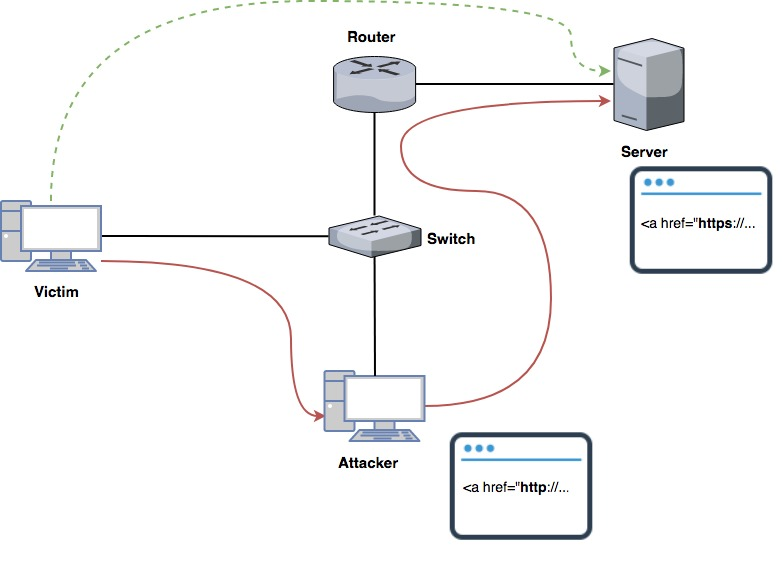
\includegraphics[width=.8\textwidth]{../figures/sslstrip}
  \caption{SSL Stripping attack diagram}
  \label{sslstrip}
\end{figure}
\begin{figure}[h]
  \center
  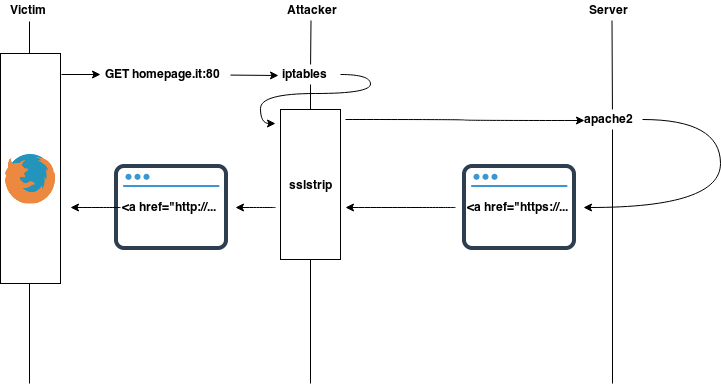
\includegraphics[width=.8\textwidth]{../figures/sslstrip_time}
  \caption{SSL Stripping attack diagram}
\end{figure}
\fxnote{avoid first person (you)}
The diagram displayed in figure \ref{sslstrip} better explain all the temporal sequence of the attack.
The user agent makes a request for a non-secure webpage, all the traffic is redirected into the attacker's virtual machine.
Using iptables you redirect all the traffic from the port 80 to the port where sslstrip is running and, then,
all the traffic is forwarded to the server. When the server response comes back,
it passes again through the proxy and all the links in the webpage get downgraded from \texttt{https://} to \texttt{http://}.
Finally, the forged webpage is returned to the user agent.
To properly mount this attack, you have to follow same specific rules:
\begin{itemize}
  \item Mount a man in the Middle attack
  \item Setup sslstrip to manipulate the HTTP traffic using this command line tool: \texttt{sslstrip -l <port>}
  \item Create a specific rule to redirect the traffic from the port 80 to the port that sslstrip is running, using iptables (mettere la riga di codice?)
  \item Navigate to \texttt{www.homepage.it} and click to the URL within the page
  \item Intercept the traffic using Wireshark and analyze the behaviour of sslstrip
\end{itemize}
\paragraph{Countermeasures}
In order to prevent this kind of attack, there is a web security policy to protect against protocol downgraded attacks, called \texttt{HTTP Strict Transport Security} (HSTS). Declaring the HSTS policy, the web server forces a browser to use HTTPS and never insecure HTTP protocol. The HSTS Policy is communicated by the server to the user agent via an HTTPS response header field named \textit{Strict-Transport-Security}.
\newpage
\subsection{Exercise 3 - HSTS Bypassing}
The HSTS policy is associated with a specific domain name and changing just by one letter the domain name, the browser will
not apply the policy anymore. For instance, an ’l’ (uncapital L) could become an ’I’ (capital i). The following diagram better shows the behaviour of this technique:
\begin{figure}[h]
  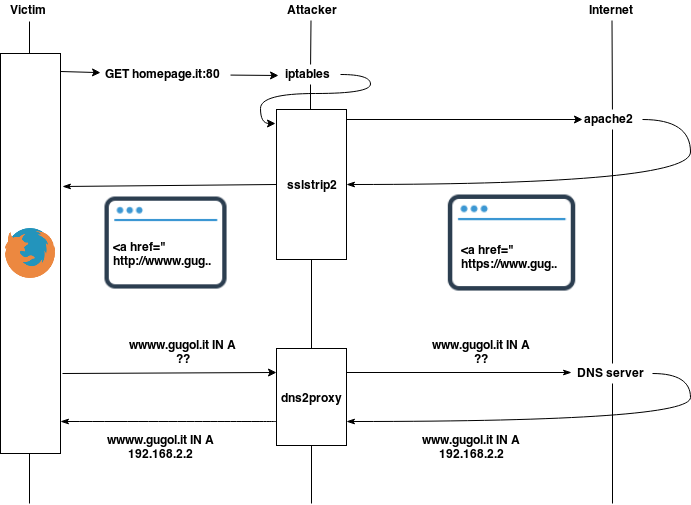
\includegraphics[width=.9\textwidth]{../figures/hsts_bypass_time}
  \caption{}
\end{figure}
\\
the first part is very similar to the one presented in the previous exercise, where all the links in the webpage get downgraded from \texttt{https://} to \texttt{http://}, adding for instance a fourth 'w' in the domain name (it can be whatever you want, the choice of adding a fourth w is due to the fact that it is not very visible).\\
When the user clicks on a link within the page the DNS queries must be manipulated as well, using the dns2proxy tool. The DNS request from the user passes through dns2proxy and is manipulated in order to be solved by the DNS server. Then, the response flows into dns2proxy again, which manipulate the response to redirect the user to a fake webpage and not to one the user was supposed to navigate.

To correctly mount this attack, you have to follow this rules:
\begin{itemize}
  \item Mount a MitM attack
  \item Implement the missing code in \texttt{sslstrip/URLMonitor.py}
  \item Create a specific rule to redirect the traffic from the port 80 to the port that sslstrip is running, using iptables (mettere la riga di codice?)
  \item Implement the missing code in \texttt{dns2proxy.py}
  \item Create a specific rule to redirect all the traffic in the attacker virtual machine changing the destination ip
  \item Analyze the behaviour using Wireshark, being sure that all this trick has being working properly
\end{itemize}
\fxnote{add the solutions}
\paragraph{Countermeasures}
Unfortunately, there is no default technique to prevent this type of attack. The user must always check the correctness of the URL in the address bar.

\end{document}
